\documentclass[a4paper,12pt]{article}
\usepackage[utf8]{inputenc}
\usepackage[french]{babel}
\usepackage[T1]{fontenc}
\usepackage{graphicx}
\begin{document}

\begin{flushleft}
GORON Nathan
\newline
L1 Informatique
\vspace{1cm}
\end{flushleft}
\begin{center}
\begin{Huge}{Guide d'utilisation : Ming-Mang}
\end{Huge}
\newline
\newline
\newline
\newline
\newline
\newline
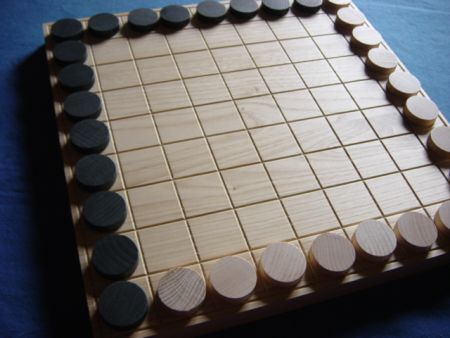
\includegraphics[scale=0.5]{images/mingmang.jpg}
\end{center}

\newpage

\section{\underline{Pré-requis système:}}
\paragraph{}
Pour lancer et utiliser le programme , vous devez avoir au préalable installé
la plus récente version de Python , il n'est nécessaire d'installer aucun module ou logiciel
additionnel .

\section{\underline{Lancement de l'application:}}
\paragraph{}
Pour utiliser l'application , ouvrer le fichier fichier "main.py" avec Idle comme
indiqué dans la capture ci dessous:
\newline
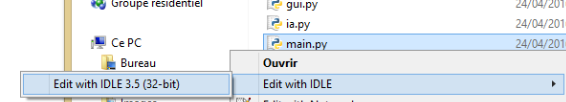
\includegraphics[scale=1]{images/lancement.png}
\newline
\paragraph{}
Une fenêtre apparait alors , appuyez sur la touche F5 pour lancer la console.
Cette console sera votre interface : vous pourrez y rentrer les commandes de jeu et
la grille apparaitra dans la boite de dialogue.\newline
Pour lancer le jeu , tapez init() dans la console , suivez ensuite les instructions qui s'affiche.
\newline
\newline
\newline

\section{\underline{Choisir son mode de jeu et jouer une partie}}
\paragraph{}
Lorsque vous aurez lancé le programme , celui-ci vous posera des questions pour définir vos préferences
, les questions seront suivis d'un code a une lettre ou a un chiffre pour définir votre réponse , exemple:
\newline
Choisissez votre mode de jeu : mode1 , mode2 , mode3 [1/2/3]
\newline 
Les choix possible apparaissent entre crochets a la fin du dialogue , tapez le chiffre ou la lettre correspondant a votre choix dans la boite de dialogue.
\newline
\newline
\newline

\section{\underline{Fonctionnalités en jeu}}
\paragraph{}
Une fois votre partie lancée , plusieurs options s'offrent a vous : Vous pouvez déplacer votre pion en suivant les instructions a dans la boite de dialogue. Vous pouvez aussi passer votre tour , pour ce faire déplacez un pion sur sa propre case en rentrant deux fois les même coordonnées .
\newline
Vous pouvez également sauvegarder une partie en tapant "save" ou "load" lorsque le programme vous propose de rentrer les coordonées d'un pion a déplacer , "save" vous permettra de sauvegarder l'état de la partie en cours(le tour ainsi que la position des pions sur le plateau) et "load" vous permettra de charger la partie sauvegardée.
\newline
\newline
\newline

\section{\underline{Utilisation de l'éditeur de plateau}}
\paragraph{}
Au lancement , le programme vous propose une set de trois variantes de jeu différentes : un plateau 9x9 , un plateau 19x19 et un plateau 29x29. Mais vous pouvez aussi créer votre propre plateau grâce a l'editeur de plateau disponible en choisissant l'option "E" lorsqu'il vous est demandé choisir la taille de votre plateau
\newline
L'application vous demandera de choisir la dimension de votre plateau puis vous pourrez placer les pions un par un comme vous le désirez. Pour terminer l'édition et lancer le jeu , tapez "jeu" au lieu de "1" ou "2" lorsqu'il vous est demandé de choisir la couleur d'un pion a placer
\newline
\newline
\newline
\section{\underline{Fin du jeu , relancement du jeu}}
\paragraph{}une fois votre partie terminée , il vous faudra fermer la console puis la relancer si vous souhaitez rejouer une partie .L'application se bloque automatiquement a la fin d'une partie et vous serez alerté par un message du gagnant et du type de victoire.



\end{document}